\section{Lösung}

In diesem Kapitel wird die geplante Lösung beschrieben, die es Nutzer:innen ermöglicht, in einer kollaborativen Umgebung Grundrisse einfach und intuitiv zu skizzieren. Ziel ist es, ein System zu schaffen, das sowohl technische Anforderungen wie Echtzeitverarbeitung und Projektion als auch nutzerzentrierte Aspekte wie Bedienbarkeit und Flexibilität berücksichtigt.

\subsection{Vision der Lösung}

Das System soll in Form eines interaktiven Tisches aufgebaut sein oder sich direkt auf einer Projektionstischfläche befinden.  
Diese physische Mitte des Workshops erlaubt allen Beteiligten, sich gleichberechtigt zu beteiligen.  
Durch die direkte Interaktion mit einem Infrarotstift können Nutzer:innen Ideen frei skizzieren, bestehende Elemente anpassen oder neue ergänzen.  
Die dabei entstehenden Änderungen werden in Echtzeit auf eine 1:1-Projektionsfläche übertragen.

Dieser Ansatz vereinfacht den Austausch, reduziert Missverständnisse und beschleunigt den Planungsprozess.  
Das System ermöglicht eine niederschwellige Beteiligung aller Workshopteilnehmenden, auch ohne technische Vorkenntnisse, und unterstützt so eine effektive und kollaborative Zusammenarbeit.





\subsection{Beobachtete Verbesserungspotenziale im Workshop}
\label{sec:verbesserungspotentiale}

Im Workshop zeigte sich deutlich, dass bestehende Methoden wie das manuelle Zeichnen auf Papier oder Bodenplänen häufig umständlich, langsam und interpretationsanfällig sind. Einzelne Beobachtungen belegen dies exemplarisch:

\begin{itemize}
  \item Ein Teilnehmer konnte eine Türrichtung nur schwer erklären. Mit einem digitalen Tool hätte er das Problem einfach aufzeigen können.
  \item Die Architektin musste physisch aufstehen, um eine Änderung im Plan vor Ort zu markieren, was den Ablauf unterbrach.
\end{itemize}

Ein digitales Zeichensystem hätte in beiden Situationen zu mehr Klarheit und Effizienz geführt.  
Zudem wurde im Rahmen des Kundeninterviews betont, dass Änderungen in einem digitalen System unmittelbar dokumentiert und als Bilddatei an die Architekt:innen weitergegeben werden können. Dadurch entfällt die Notwendigkeit, zunächst einen schriftlichen Bericht zu verfassen, was den Kommunikations- und Entscheidungsprozess erheblich beschleunigt.
\clearpage

\subsection{User Story - vorher und nachher}

Um den Mehrwert der entwickelten Lösung greifbar zu machen, werden im Folgenden zwei beispielhafte Szenen gegenübergestellt: einmal ohne unterstützendes Zeichentool und einmal mit der neuen Anwendung. 

Das dargestellte Szenario basiert auf einem realen Workshop mit dem Wohnheim Humanitas am SCDH. Dort wurde gemeinsam mit Pflegefachkräften und Architektinnen ein konkreter Fall aus dem Pflegealltag simuliert und analysiert.

\subsubsection*{Vorher: Ohne digitale Unterstützung}

\textbf{Teilnehmer:} Pflegefachkraft, Architektin, Workshop-Moderator

Während des Szenarios wurde deutlich, dass die Tür zwischen einem Pflegezimmer und dem angrenzenden Duschraum nach aussen öffnet. Diese öffnet sich in die Richtung der ankommenden Person. Eine Pflegefachkraft wies darauf hin, dass dies im Pflegealltag hinderlich sei, insbesondere beim Schieben eines Rollstuhls oder Pflegebetts, da der Türflügel den Durchgang blockieren kann. Der Teamleiter griff das Anliegen auf und brachte es im abschliessenden Debriefing zur Sprache.

In der anschliessenden Diskussion mit den Architektinnen und Architekten zeigte sich, dass eine Öffnung nach innen aus baulichen Gründen nicht realisierbar ist. Es entstand die Idee, von einer linksöffnenden zu einer rechtsöffnenden Tür zu wechseln.

Der Workshop-Moderator versuchte daraufhin, die Situation mithilfe eines digitalen Plans auf dem Präsentationsbildschirm am vorderen Ende des Raums zu skizzieren. Da er die räumlichen Ausführungen jedoch nicht vollständig verstanden hatte, war er nicht in der Lage, die Änderung gemäss der Vorstellung der Teilnehmenden einzuzeichnen. Dies führte zu Verwirrung, Rückfragen und Verzögerungen, welche den Gesprächsverlauf merklich störten.

\begin{figure}[H]
    \centering
    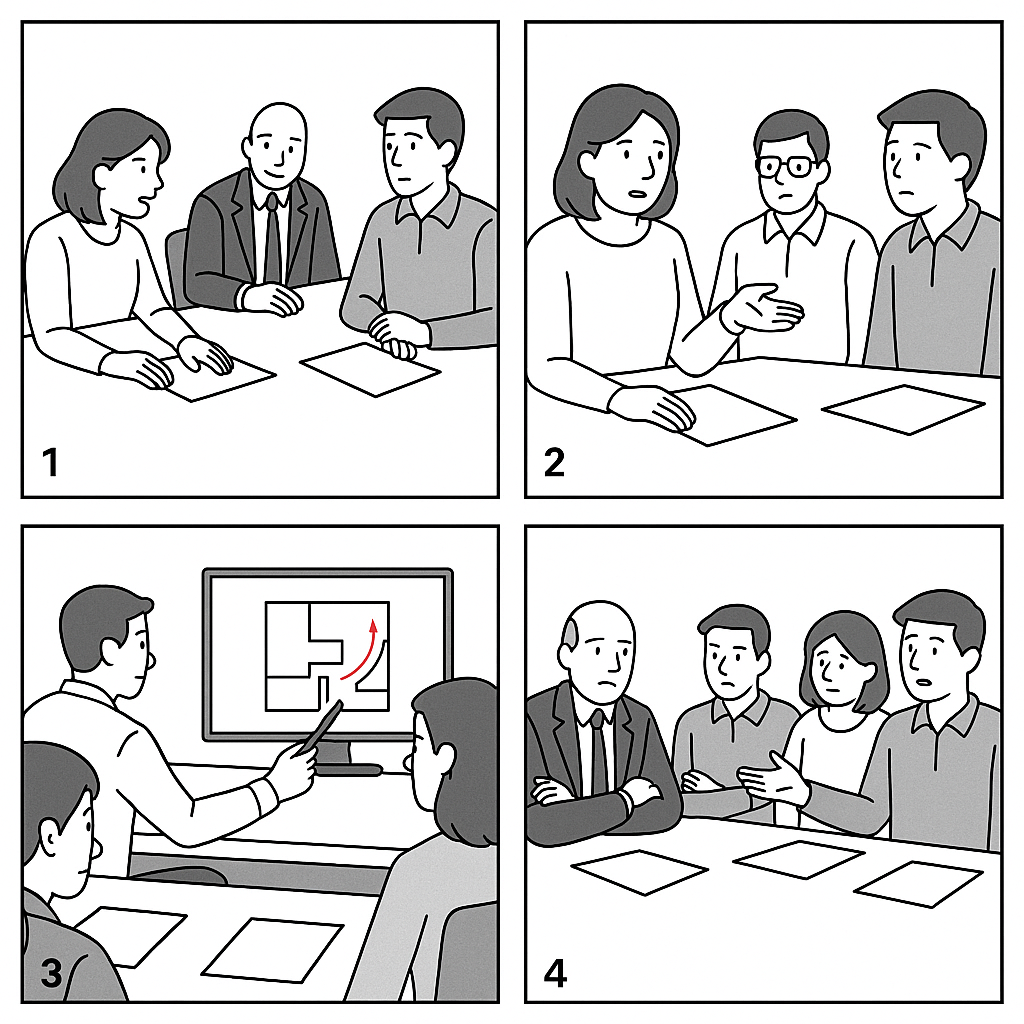
\includegraphics[width=0.75\textwidth]{graphics/UserStory_without_Solution.png}
    \caption{Storyboard ohne digitales Zeichentool}
    \label{fig:userstory-ohne}
\end{figure}

\textbf{Legende:}
\begin{itemize}
    \item \textbf{Panel 1:} Eine Pflegefachkraft spricht ein von ihr erkanntes Problem an.
    \item \textbf{Panel 2:} Die Architektin sitzt am Tisch und schaut fragend. Ihre Körperhaltung zeigt Unklarheit über das geschilderte Problem.
    \item \textbf{Panel 3:} Die Diskussion ist unterbrochen. Der Moderator sitzt allein vor dem Desktop. Er blickt konzentriert, aber unsicher auf den Bildschirm und arbeitet an der Visualisierung.
    \item \textbf{Panel 4:} Die Gruppe blickt auf den Bildschirm. In den Gesichtern ist Irritation erkennbar. Die vom Moderator erstellte Visualisierung entspricht nicht dem Problem der Pflegefachkraft.
\end{itemize}

\clearpage

\subsubsection*{Nachher: Mit digitalem Zeichentool}

\textbf{Teilnehmer:} dieselben Rollen wie zuvor

 Die Anwendung erlaubt es, mithilfe eines Infrarotstifts intuitiv auf einer horizontalen Projektionsfläche zu zeichnen. Die Eingaben werden in Echtzeit erkannt und visuell hervorgehoben. Mit diesem neuen digitalen Zeichentool hätte jede beteiligte Person, zum Beispiel die Pflegefachkraft oder der Teamleiter, die räumliche Problematik direkt auf dem projizierten Grundriss auf dem Tisch visualisieren können.

\begin{itemize}
    \item Position der betroffenen Tür
    \item Richtung der Türöffnung
    \item Bewegungsweg der Pflegeperson
\end{itemize}

Alle relevanten Informationen wären direkt für alle Beteiligten sichtbar gewesen.  
Die Darstellung auf der gemeinsamen Tischprojektion hätte es ermöglicht, räumliche Situationen live zu erfassen und gemeinsam zu diskutieren.  
Die Auswirkungen der Türöffnung auf die Bewegungssituation wären unmittelbar nachvollziehbar gewesen.

Im weiteren Verlauf hätte die Architektin anhand der markierten Türposition und Öffnungsrichtung rasch erkannt, worin das Problem besteht.
Alle Änderungen an der Türposition oder der Türöffnungsrichtung hätten direkt und unmissverständlich visualisiert, gemeinsam diskutiert und auf ihre Umsetzbarkeit überprüft werden können.

Die Diskussion wäre visuell unterstützt, interaktiv und zielgerichtet verlaufen.  
Fehlinterpretationen und Missverständnisse, wie sie im ursprünglichen Szenario auftraten, wären vermieden worden.  
Darüber hinaus hätte das System die erarbeitete Skizze automatisch dokumentieren und als Datei weitergegeben werden können, ohne zusätzliche Nachbearbeitung.

\begin{figure}[H]
    \centering
    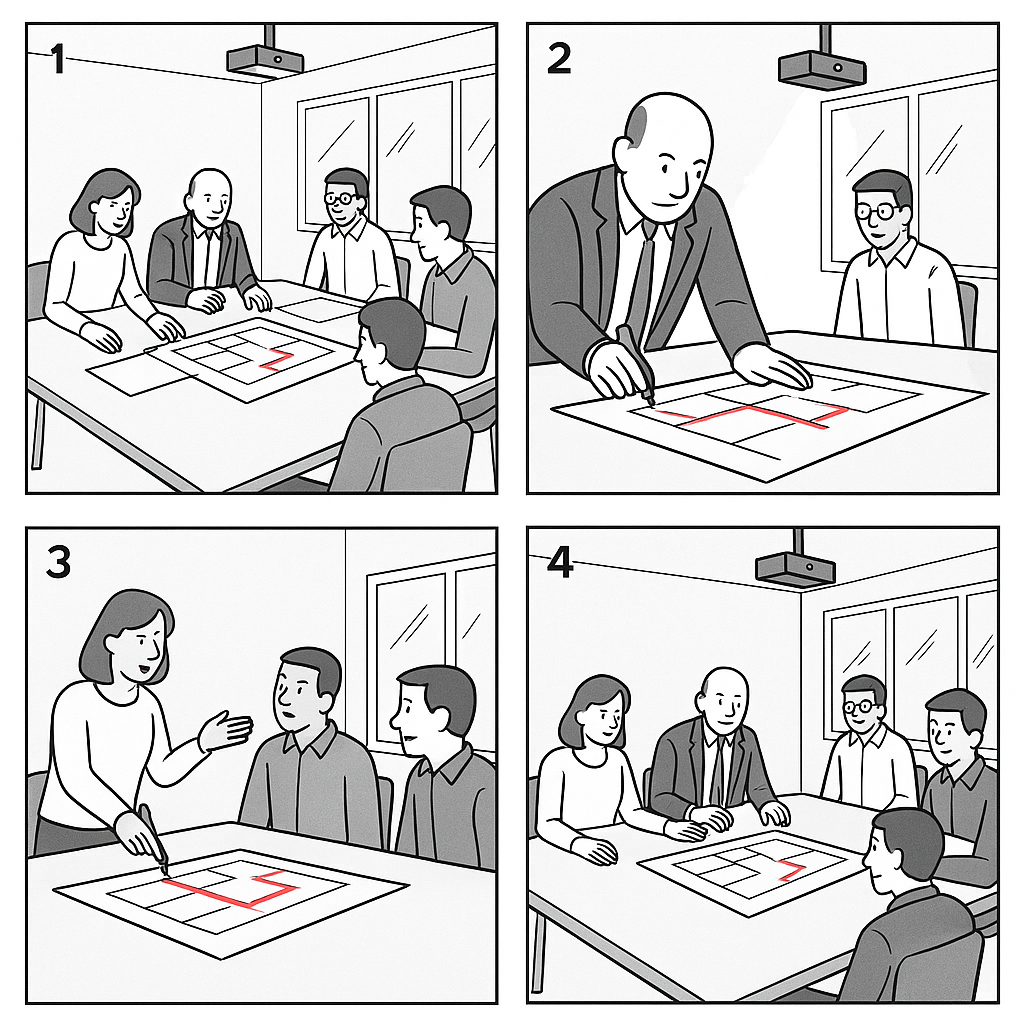
\includegraphics[width=0.75\textwidth]{graphics/UserStory_with_Solution.png}
    \caption{Storyboard mit digitalem Zeichentool}
    \label{fig:userstory-mit}
\end{figure}

\textbf{Legende:}
\begin{itemize}
    \item \textbf{Panel 1:} Die Beteiligten sitzen gemeinsam um den interaktiven Tisch. Der Grundriss wird auf die Tischfläche projiziert. Die Szene leitet die Diskussion zur Türsituation ein.
    \item \textbf{Panel 2:} Die Türposition und ihre Öffnungsrichtung werden deutlich sichtbar (in rot) auf dem Plan eingezeichnet. Alle Beteiligten blicken darauf.
    \item \textbf{Panel 3:} Die Architektin hebt die Hand und bringt sich aktiv ein. Ihr Gesichtsausdruck zeigt, dass sie das Problem nachvollziehen kann.
    \item \textbf{Panel 4:} Zwei Personen deuten auf den Plan. Die Diskussion ist im Gange, die vorgeschlagene Lösung wird gemeinsam reflektiert.
\end{itemize}


\clearpage


\subsection{Verknüpfung mit den Forschungsfragen}

Die in diesem Kapitel dargestellten Herausforderungen und Lösungsansätze lassen sich klar auf die im Projekt definierten Forschungsfragen beziehen:

Die Beobachtungen im Workshop, insbesondere die erschwerte Kommunikation räumlicher Probleme und die mangelnde Flexibilität bei Änderungen, unterstreichen die Relevanz von \textbf{Forschungsfrage 1}, in der untersucht wird, \textit{wie ein System gestaltet werden kann, das eine einfache und kollaborative Planung von Grundrissen ermöglicht}. Unsere Lösung adressiert diese Problematik durch die Kombination eines intuitiven Zeichensystems mit direkter Projektion.

Bezüglich \textbf{Forschungsfrage 2} \textit{wie die Benutzeroberfläche trotz Funktionsreichtum verständlich und intuitiv für Laien gestaltet werden kann} wurde bei der Systemgestaltung besonders auf eine stiftbasierte Eingabe gesetzt. Diese ist für Nutzer:innen vertraut und benötigt keine Schulung oder erklärende Bedienkonzepte.

Schliesslich zielt \textbf{Forschungsfrage 3} darauf ab, zu verstehen, \textit{wie die Lösung in realen Workshops hinsichtlich Usability, Zusammenarbeit und Flexibilität wahrgenommen wird}. Die im Workshop beobachteten Situationen zeigen deutlich, dass ein visuelles Live-Tool den Diskussionsfluss verbessert, die Beteiligung aller fördert und sich flexibel an unterschiedliche Anforderungen des SCDH anpassen lässt. Zudem gibt eine digitale Lösung den Teilnehmenden die Sicherheit, dass ihre Inputs direkt und korrekt erfasst werden und nicht bei der Protokollierung verloren gehen oder später fehlinterpretiert werden.

Damit wird deutlich, dass die Systemgestaltung nicht isoliert entstanden ist, sondern direkt aus den praktischen Bedürfnissen und Anforderungen des Projektkontexts abgeleitet wurde.
